\documentclass[12pt]{amsart}
\usepackage{setspace}
\doublespacing
\textwidth=5.5in

\usepackage{graphicx}
\usepackage{placeins}
\usepackage{amsmath}
\usepackage{hyperref}
\usepackage{ amssymb }
\usepackage{longtable}

\newcommand{\iid}{\stackrel{iid}{\sim}}
\newcommand{\trip}[3]{#1_{#2}^{(#3)}}
\newcommand{\bb}[1]{\mathbf{#1}}
\newcommand{\z}{\mathbf{z}}
\newcommand{\w}{\mathbf{w}}
\newcommand{\X}{\mathbf{X}}
\newcommand{\Y}{\mathbf{Y}}
\newcommand{\myn}[3]{n_{#1,#2}^{(#3)}}
\newcommand{\Rea}{\mathbb{R}}
\newcommand{\topics}{\text{ topics }}

\title{$R^2$ For Topic Models}
\author{Thomas W. Jones}
\begin{document}
\maketitle

\begin{abstract}
This document proposes a new (old) metric for evaluating goodness of fit in topic models, the coefficient of determination, or $R^2$.
\end{abstract}

\section{Introduction}

\section{Probabilistic Topic Models}
Probabilistic topic models are a family of stochastic models for estimating abstract ``topics" in a set of documents. Many topic models have been developed and provide a flexible family of topic models. Some include frequently available metadata about documents, such as the time of the publication in Dynamic Topic Models, or the author and location of the publication. Most topic models are Bayesian, though probabilistic latent semantic analysis (pLSA), wich is sometimes called probabilistic latent semantic indexing (pLSI) is frequentist. All probabilistic topic models share common features. Without loss of generality: all topic models model documents as a mixture of categorical distributions.\footnote{For estimation purposes, these are really multinomial distributions with $N_d$ being the number of words in each document. Adding confusion, the terms ``multinomial" and ``categorical" are often used interchangeably in the literature.} The goal of topic modeling is to estimate the parameters of these distributions. The most basic kind of topic model is parameterized as follows:

\begin{align*}
Z_d \sim& Categorical_K({\theta}_d) && d\in \{1, \ldots, D\}\\
V_k \sim& Categorical_V({\phi}_{k}) && k\in \{1, \ldots, K\}\\
\end{align*} where $Z_d$ represents topics over documents, $V_k$ represents words over topics, $K$ is the number of latent factors or ``topics", $V$ is the number terms in the model and indexed by $v \in \{1, \ldots, V\}$, and $N_d$ is the number of terms in the $d^{th}$ document. Latent Dirichlet allocation (LDA), possibly the most popular topic model, places Dirichlet priors on $\theta_d, \forall d$ and $\phi_k, \forall k$:
 
\begin{align*}
\phi_k \sim& Dirichlet_V(\beta) && k\in\{1, \ldots, K\} \\
{\theta}_d \sim& Dirichlet_K({\alpha}) && d\in\{1, \ldots, D\}\\
\end{align*}

A topic model's estimates are generally represented in two matrices., $\Theta$ and $\Phi$. The $d$-th row of $\Theta$ is $\theta_d$, whose $k$-th entry is the probability of topic $k$ conditional on document $d$. The $k$-th row of $\Phi$ is $\phi_k$, whose $v$-th entry is the probability of word $v$ conditional on topic $k$. The document term matrix $Y$ can be thought of as the result of repeated sampling from $\Theta$ and $\Phi$. The dot product of $\Phi$ and $\Theta$ is the expected value of the document term matrix: $E(Y) = \Theta^T\Phi$. 

\section{Goodness-of-Fit For Topic Models}

According to an often-quoted but never cited definition, ``the goodness of fit of a statistical model describes how well it fits a set of observations. Measures of goodness of fit typically summarize the discrepancy between observed values and the values expected under the model in question."\footnote{This quote appears verbatim on Wikipedia and countless books, papers, and websites.} Goodness of fit is not the only consideration in statistical modeling. In a model predicting cancer recurrence rates, for example, researchers' primary concern is likely which predictors are most associated with cancer recurrence, rather than explicit prediction for future patients. However, goodness of fit is a key metric in establishing trust in a model. If an easily-interpreted model does not fit the data well, it cannot be trusted for inference.\footnote{The opposite is not necessarily true; interpretability is not necessary for accurate prediction.} Certain processes are noisier than others, making goodness of fit more or less important. Consider the difference between financial models and microeconomic models. In finance, the high variability of the data makes an $R^2$ of $0.1$ relatively high. In microeconomics, however, an $R^2$ of $0.1$ is not compelling. Many accurate and robust predictive models are ``black boxes", making inference difficult. Researchers may trade off some goodness of fit for interpretability. However, the model must still fit the data reasonably well if inferences are to be convincing. This tension between interpretability and goodness of fit is present in topic modeling


Topic models are generative models of word frequency. For a set of learned distributions of topics and topic proportions, denoted by $\hat{\phi_k}$ and $\hat{\theta_d}$, 

\section{Review: $R^2$ for the General Case}

The common definition of $R^2$ is a ratio of sums of squared errors. 
\begin{align*}
    R^2 \equiv 1 - \frac{SS_{resid.}}{SS_{tot.}}
\end{align*} For a model, $f$, of outcome variable, $y$, where there are $n$ observations, $R^2$ is derived as follows:

\begin{align*}
	& \text{The mean of the data is} & \bar{y} &= E(y) \\ %\frac{1}{n}\sum_{i=1}^n{y_i}\\
	& \text{The total sum of squares is} & SS_{tot.} &= \sum_{i-1}^n{(y_i-\bar{y})^2}\\
	% & \text{The model sum of squares is} & SS_{model} &= \sum_{i-1}^n{(f_i-\bar{y})^2}\\
	& \text{The residual sum of squares is} & SS_{resid.} &= \sum_{i-1}^n{(f_i-y_i)^2}\\
	& \text{Finally, the coefficient of determination is} & R^2 &\equiv 1 - \frac{SS_{resid.}}{SS_{tot.}}\\
\end{align*}

$R^2$, as defined above, is bound between 0 and 1 when $f$ is a linear model. If $f$ is not linear, then negative values of $R^2$ are possible. In this case, $SS_{resid.}$ may be larger than $SS_{tot.}$ and then $R^2$ may be negative. However, when $f$ perfectly fit the data, $f_i=y_i\forall i $ and $SS_{resid}=0$. In this case, $R^2$ is equal to one. 

In some cases, $SS_{tot.}$ can be partitioned into two parts, $SS_{tot.} = SS_{resid.} + SS_{model}$. $SS_{model}$ is the model sum of squares: $SS_{model} = \sum_{i-1}^n{(f_i-\bar{y})^2}$. When this relation holds, then $R^2$ is interpreted as the proportion of variance of $y$ explained by $f$. This is derived below.\footnote{TOMMY, YOU NEED A REFERENCE FOR THIS AS THIS DERIVATION DOES NOT PROVE THAT $E(f) = y$. Also, does this interpretation hold in the Bayesian case? Must investigate.}

\begin{align*}
V(f) &= E((f - E(f))^2)\\
     &= E((f - E(y))^2)\\
     &= E((f - \bar{y}))\\
     &= \frac{1}{n}\sum_{i-1}^n{(f_i-\bar{y})^2}\\
     &= \frac{1}{n}SS_{model}\\
V(y) &= E((y - E(y))^2)\\
     &= E((y - \bar{y})^2)\\
     &= \frac{1}{n}\sum_{i-1}^n{(y_i-\bar{y})^2}\\
     &= \frac{1}{n}SS_{tot.}\\
\frac{V(f)}{V(y)} &= \frac{SS_{model}/n}{SS_{tot.}/n}\\
     &= \frac{SS_{model}}{SS_{tot.}}\\
     &= 1 - \frac{SS_{resid.}}{SS_{tot.}} \text{\footnote{This holds because $SS_{tot.} = SS_{model} + SS_{resid.} \Rightarrow \frac{SS_{model}}{SS_{tot.} + \frac{SS_{resid.}}{SS_{tot.}} = 1}$}}\\
     &\equiv R^2
\end{align*}

\section{ A Geometric Interpretation of $R^2$}
$R^2$ has a geometric interpretation. As we will see later, this interpretation applies to an $R^2$ for topic models. $SS_{tot.}$ is the total squared-euclidean distance from each $y_i$ to the mean outcome, $\bar{y}$. Then $SS_{resid.}$ is the total squared-euclidean distance from each $y_i$ to its predicted value under the model, $f_i$. Recall that for any two points $p, q \in \mathbb{R}_m$

\begin{align*}
	d(p,q) = \sqrt{\sum_{j=1}^m{(p_j - q_j)^2}}\\
\end{align*} where $d(p, q)$ denotes the euclidean distance between $p$ and $q$. $R^2$ is often taught in the context of ordinary least squares (OLS) where $y_i, f_i \in \mathbb{R}_1$. In that case, $d(y_i, f_i) = \sqrt{(y_i - f_i)^2}$; by extension $d(y_i, \bar{y}) = \sqrt{(y_i - \bar{y})^2}$.\footnote{In the one-dimensional case, where $y_i , f_i \in \mathbb{R}_1$, $SS_{resid.}$ can be considered the squared-euclidean distance between the $n$-dimensional vectors $y$ and $f$. However, this relationship does not hold when $y_i , f_i \in \mathbb{R}_m ; m > 1$.} In the multidimensional case where $y_i, f_i \in \mathbb{R}_m; m > 1$, then $\bar{y} \in \mathbb{R}_m$ as well. Here, $\bar{y}$ represents the point at the center of $y$ in $m$ space.

We can rewrite $R^2$ using the relationships above. 

\begin{align*}
    SS_{tot.} &= \sum_{i=1}^n{d(y_i, \bar{y})^2}\\
    SS_{resid.} &= \sum_{i=1}^n{d(y_i, f_i)^2}\\
    \Rightarrow R^2 &= 1 - \frac{\sum_{i=1}^n{d(y_i, f_i)^2}}{\sum_{i=1}^n{d(y_i, \bar{y})^2}}
\end{align*}


If SSR > SST, then f = ybar is a better predictor than my model. In this case, R2 is negative.

If SSR = SST, then my model is just as good as guessing ybar.

If SSR = 0, then my model is a perfect fit for the data.

If 0 < SSR < SST, then my model is a better fit for the data than just guessing ybar.

\begin{figure}
\centering
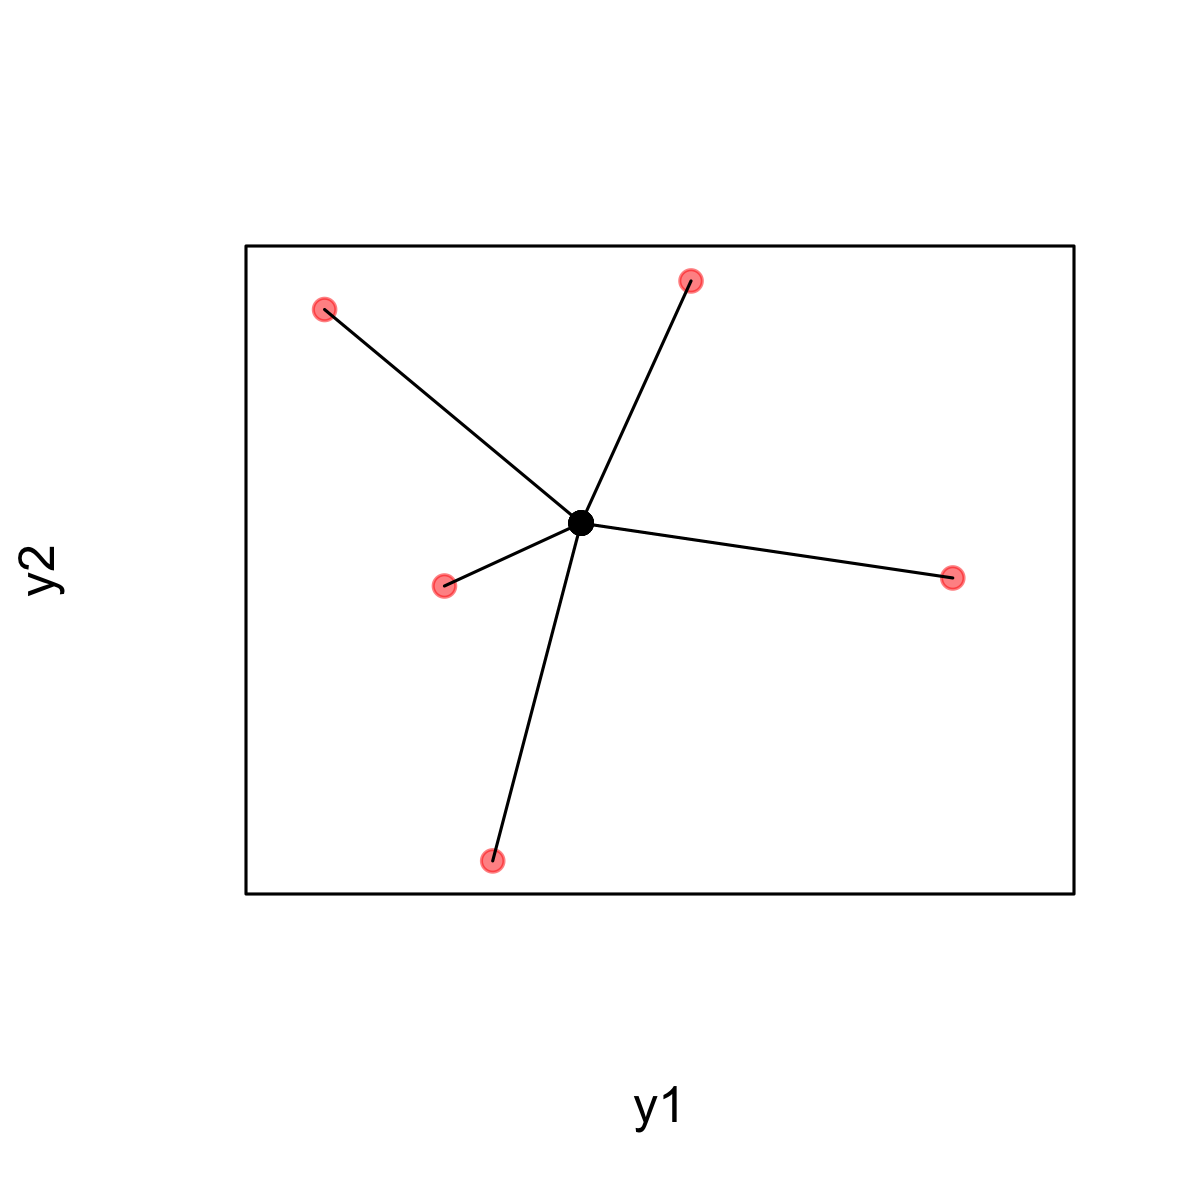
\includegraphics[scale=0.15]{{output/geometric1.png}} 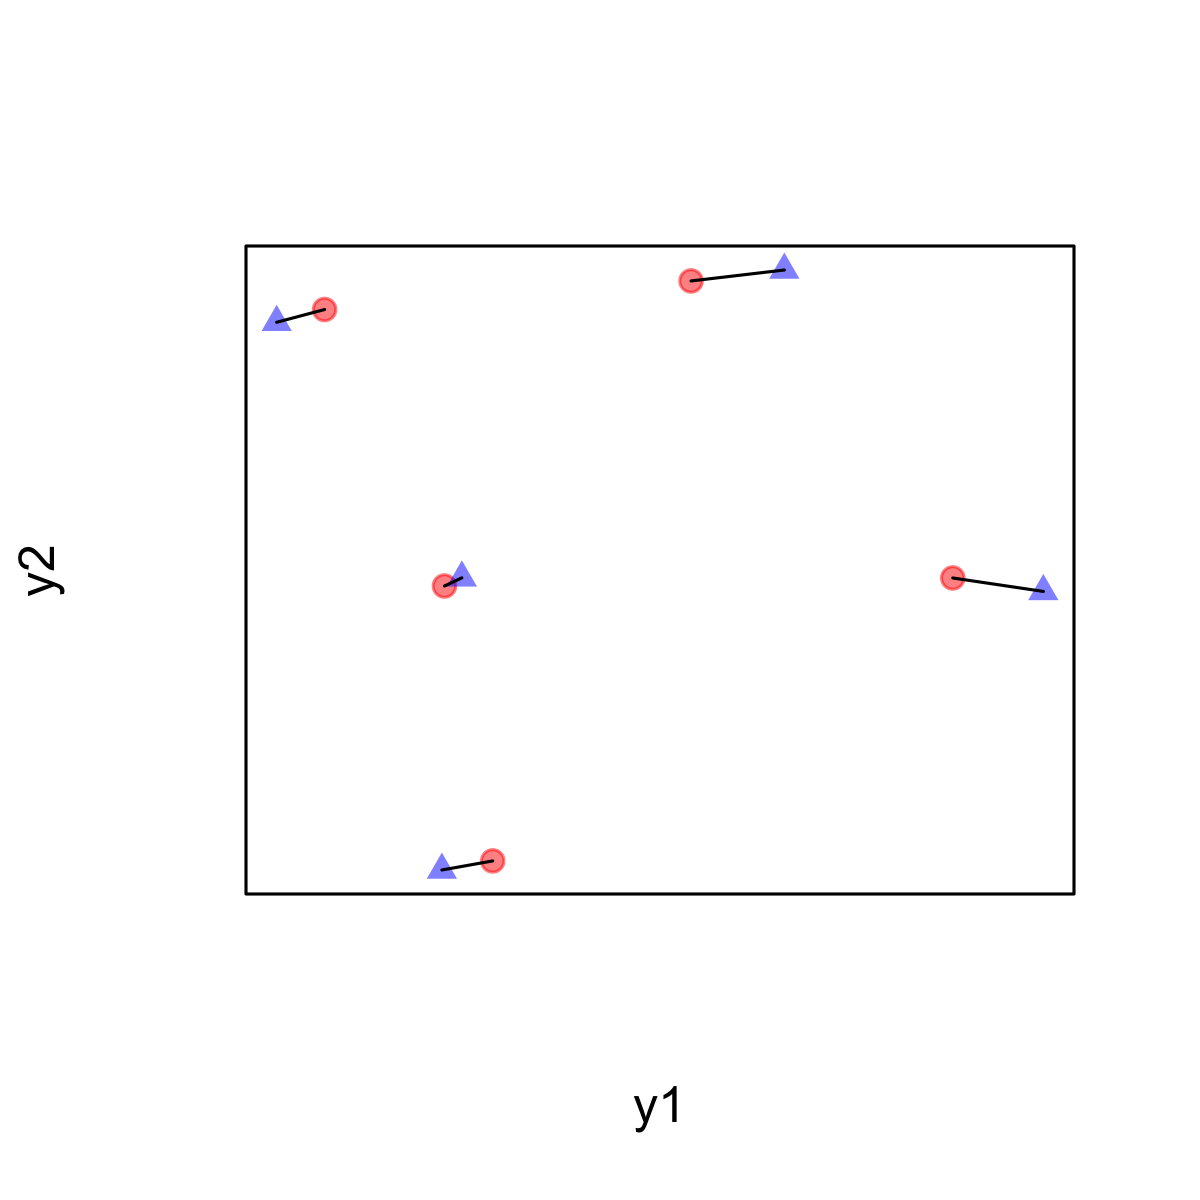
\includegraphics[scale=0.15]{{output/geometric2.png}}
\caption{The figure on the left depicts... the figure on the right depicts...}
\end{figure}

%"Coefficient of Determination" by Orzetto - Own work. Licensed under CC BY-SA 3.0 via Wikimedia Commons - http://commons.wikimedia.org/wiki/File:Coefficient_of_Determination.svg#mediaviewer/File:Coefficient_of_Determination.svg
\section{$R^2$ For Topic Models}



\section{Conclusion}




\section{Appendix}

\newpage
\begin{thebibliography}{9}

 

\end{thebibliography}


\end{document}